%\documentclass[handout,aspectratio=169]{beamer} %in pdf pro Folie eine Seite - dies verwenden, wenn der Vortrag nachträglich den Teilnehmern zur Verfügung gestellt wird
\documentclass[aspectratio=169]{beamer} %in pfd pro animierten Klick eine Seite  - dies für die Präsentation verwenden
% aspectratio=169 bedeutet 16:9 Format

%*************************************************************************************************************
%%%packages

%Mathematik:
\usepackage{amsmath}
\usepackage{amsthm}
%Umlaute tippen
\usepackage[utf8]{inputenc}
%Wörterbuch für korrekte Silbentrennung
\usepackage[ngerman]{babel}
% für Algorithmus
\usepackage[noend]{algorithmic}
\usepackage{algorithm}
%Blockweises auskommentieren mit \begin{comment}\end{comment}
\usepackage{verbatim}
%Farben
\usepackage{xcolor}
%Icons
\usepackage{fontawesome5}
%Grafiken 
\usepackage{graphicx} %Bilder einbilden
\graphicspath{{bilder/}} %Es gibt ein Unterverzeichnis, wo alle Bilder liegen. Durch diesen Befehl muss man nicht jedes mal den Dateipfad angeben


%tikz
\usepackage{tikz} %Grafiken erstellen
\usetikzlibrary{arrows,automata}
%Styles definieren
\tikzset{>=stealth, shorten >= 1pt,auto}
\tikzstyle{initial}+=[initial text=]

%Literaturverzeichnis (wenn nicht auf jeder Seite ein einzelnes Verzeichnis)
\usepackage{biblatex}
\usepackage{csquotes}
\bibliography{bibliography} %bib-Dokument referenzieren
%*************************************************************************************************************

%%%%%%%% Layout %%%%%%%%

\usetheme[]{Boadilla}
%\usecolortheme{rose}% schwache Farben
% Themes:
%AnnArbor | Antibes | Bergen |Berkeley | Berlin | Boadilla |boxes | CambridgeUS | Copenhagen |Darmstadt | default | Dresden |
%Frankfurt | Goettingen |Hannover | Ilmenau | JuanLesPins | Luebeck | Madrid | Malmoe | Marburg | Montpellier | PaloAlto | Pittsburgh |Rochester | Singapore | Szeged |Warsaw
\useinnertheme{rounded}
%\useoutertheme{shadow}% Schattierung in den Rechtecken der Blöcken
\beamertemplatenavigationsymbolsempty% Navigationssymbole sollen ausgeblendet werden

%Fußzeile
\setbeamertemplate{footline}{
	\hfill%
	%Nur die Seitenzahlen in der Fußzeile:
	\usebeamercolor[fg]{page number in head/foot}%
	\usebeamerfont{page number in head/foot}%
	\setbeamertemplate{page number in head/foot}[framenumber]%
	\usebeamertemplate*{page number in head/foot}\kern1em\vskip2pt%
}

%*************************************************************************************************************

%%% Informationen für Titelseite
\title[Short Title]{Long Title}
\author[Lastname]{Full name} 
\institute{TU Dortmund}
\date{\only<0|handout:1>{Last Update: \today}}% das Datum wird nur im handout-modus angezeigt

%*************************************************************************************************************

%%%Folien 
\begin{document}

%%Titelfolie	
\begin{frame}[plain, noframenumbering]%Titelseite soll nicht in die Seitenzahlen mitgezählt werden
    \titlepage
\end{frame}

\section{Texte}

\begin{frame}{Texte und Formeln}
	\only<1,3>{Dieser Text erscheint nur auf Folie 1 und 3.\newline}
	\visible<2->{Ab Folie 2 stellen wir Formeln vor: \newline
	Es gibt eingerückte Formeln im display math mode  \[a = b + c\] und Formeln innerhalb des Textes im math mode $c = b$.}
\end{frame}

\begin{frame}{Auflistung}
	Hier folgt eine nummerierte Auflistung:
	\begin{enumerate}
		\item Text kann schrittweise enthüllt werden \pause 
		\item Aber bitte \pause nicht zu \pause kleinschrittig!
	\end{enumerate}
	
	Hier folgen Stichpunkte:
	\begin{itemize} %an der folgenden nötigen Nummerierung der "Klicks" sieht man, dass es ungünstig ist, \pause und <number> zu kombinieren
	\item sichtbar sobald \texttt{$\backslash$pause}-Aufklappen hier angekommen
	\item<5-> sichtbar ab Folie 5
	\item<5-7> sichtbar auf den Folien 5-7
	\item<6> sichtbar nur auf Folie 6
	\end{itemize}
\end{frame}

\begin{frame}{Blöcke}
	\begin{exampleblock}{Ein Beispielblock}
		Text des Beispielblocks
	\end{exampleblock}
	\begin{alertblock}{Hervorgehobener Block}
		Ist das wirklich so wichtig?
	\end{alertblock}
	\begin{definition}
		Text der Definition
	\end{definition}
	\begin{theorem}[Titel des Theorems]
		Aussage des Theorems
	\end{theorem}
\end{frame}

\section{Grafiken}

\begin{frame}{Bilder}
	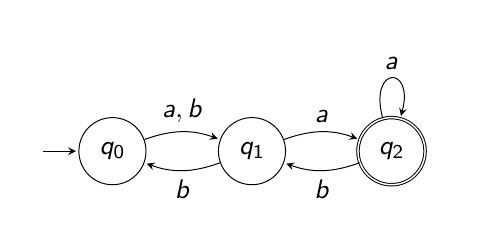
\includegraphics[width=\linewidth]{automat.jpg} 
	%\linewidth= geht über die gesamte Breite, Höhe wird automatisch skaliert 
\end{frame}

\begin{frame}{tikz-Grafiken}
	\centering %das folgende wird zentriert
		
	\begin{tikzpicture}[scale= 2.5]% Das Bild wird um das 2.5-Fache vergrößert
		\node[state, initial] (0) at (0,0){$q_0$};
		\node[state] (1) at (2,0) {$q_1$};
		\node[state, double] (2) at (4,0) {$q_2$};
		\only<1>{ %auch in Grafiken können Elemente animiert werden
			\draw[->] (0) edge[bend left=20] node[auto] {$a,b$} (1);}
		\visible<2->{
			\draw[->] (1) edge[bend left=20] node[auto] {$a$} (2)
			edge[bend left=20] node[auto] {$b$} (0);}
		\invisible<3>{
			\draw[->] (2) edge[loop above] node[auto] {$a$} ()
			edge[bend left=20] node[auto] {$b$} (1);}
	\end{tikzpicture}
\end{frame}

\section{Literaturangaben}

\begin{frame}{Quellenverzeichnis auf der jeweiligen Folie}
	
	Für wichtige Quellen bietet es sich an, diese auf der jeweiligen Folie zu nennen, da die Zuhörer nicht bei Bedarf während des Vortrages zum Quellenverzeichnis springen können. Grundsätzlich müssen in einem Vortrag nicht alle Referenzen angegeben werden! Wenn sich jemand für die genaue Quelle einer Aussage interessiert, könnt ihr auf das Literaturverzeichnis am Ende oder Eure Ausarbeitung verweisen.
	
	Für das gegebene Code-Beispiel muss pro frame eine Quelle aber immer neu eingepflegt werden, das kann umständlich und fehleranfällig sein!
	
	\let\thefootnote\relax\footnotetext{\faBook~  M. de Berg, \emph{Robot Motion Planning}, in \emph{Computational geometry}, 1997}
\end{frame}

\begin{frame}{Zusammenfassung und offene Fragen}
	Eure Abschlussfolie sollte den Inhalt der Präsentation zusammenfassen und anregend für Fragen \& Diskussion sein.
\end{frame}

\begin{frame}[plain,noframenumbering,allowframebreaks]{Quellenverzeichnis}%Falls das Verzeichnis zu lang wird, wird auf der nächsten Seite automatisch fortgeführt, Literaturverzeichnis soll nicht in die Seitenzahlen mitgezählt werden
	\nocite{*}%das ganze Literaturverzeichnis wird angegeben, egal ob die Quelle im Dokument zitiert wird oder nicht
	\printbibliography
\end{frame}

\end{document}
